\documentclass[conference]{IEEEtran}

\usepackage[utf8]{inputenc}
\usepackage[T1]{fontenc}
\usepackage[english]{babel}
\usepackage{microtype}
\usepackage{amsmath,amssymb}
\usepackage{graphicx}
\graphicspath{{figs/}}
\usepackage{booktabs}
\usepackage{url}
\usepackage{xcolor}
\usepackage[colorlinks=true,urlcolor=blue,citecolor=black,linkcolor=black]{hyperref}

\begin{document}

\title{Raft and Fault-Tolerant Key/Value Storage}

\author{
\IEEEauthorblockN{Everton Romanzini Colombo}
\IEEEauthorblockA{\texttt{e257234@dac.unicamp.br}}
\and
\IEEEauthorblockN{Henrique Ribeiro Medeiros da Silva}
\IEEEauthorblockA{\texttt{h243172@dac.unicamp.br}}
}

\maketitle

\section{Introduction}
Replicating a service across several machines is a standard way to make systems resilient to faults, but copying alone is not enough:
the replicas must agree on a single order of operations so that all copies stay identical, and they must keep agreeing while the network drops or delays messages,
or while replicas crash and later rejoin the cluster.
Many consensus algorithms solve this problem by having every replica apply the same log of commands. The Raft algorithm~\cite{raft2014} is one of them:
it was designed to be easy to understand and is the basis of many production systems, including etcd, Consul, and CockroachDB\@.

Raft's fault tolerance comes at a cost, however. Every operation must reach a majority of the replicas before it is answered, so that it is not lost if a minority of them crash,
and waiting for them over the network costs throughput and latency. Moreover, Raft keeps that single order by routing all client requests through one leader replica, so when the leader crashes,
the service stops until the other replicas elect a new one.

With this in mind, this project had two main parts: (1) implementing Raft and a simple key/value storage system on top of it to understand the protocol in detail,
and checking it against the extensive test suite of MIT's 6.824 course~\cite{mit6824};
and (2) automating experiments to measure the cost of fault tolerance in a containerized deployment. Together, these parts cover key distributed systems topics such as leader election, consensus,
replication, consistency, and failure detection.

The project repository can be accessed \href{https://github.com/Everton-Colombo/raft_and_kv-raft}{here}, and a demonstration video \href{https://youtu.be/8nt4VyT0qKw}{here}.

\subsection*{Basis and scope}
This project's starting point was the framework of MIT's 6.824 course (2020)~\cite{mit6824}, specifically labs 2 (Raft) and 3 (a key/value service on top of it), which supplied, crucially,
a thorough set of tests, along with what they need to run: the function signatures they call, a simulated in-memory network on which they inject faults,
and the Porcupine linearizability checker~\cite{porcupine}. The Raft and key/value implementations are ours, as are the deployment and experiments built around them.
Appendix~\ref{sec:algs-reuse} lists exactly what was kept, changed, and written. Concretely, we built:

\begin{itemize}
\item \textbf{Raft}, with leader election, log replication, persistence and snapshots, closely following the Raft paper~\cite{raft2014}.
\item \textbf{Key/Value Service}, built on top of our Raft implementation, with clients that find the current leader and resend their request when it changes,
a response cache that keeps retried requests from being applied twice, and snapshots of its state that replace the log entries already applied so that the Raft log does not grow forever.
\item \textbf{Container Deployment}, which uses a Dockerfile and \texttt{compose.yaml} to run every replica from the same image, each in its own container,
with environment variables that give each replica its ID, the other replicas' addresses and where to store its state.
\item \textbf{HTTP Interface}, through which clients reach the service, plus a \texttt{/status} endpoint that reports each replica's term, leader and log position.
\item \textbf{Experiments}, driven by a script that crashes, disconnects or slows down replicas while a benchmark client measures throughput and latency.
This client uses Porcupine to check that the service stays linearizable, and the script also queries \texttt{/status} every 50\,ms to measure how long elections and recovery take.
\end{itemize}

The remainder of this report is organized as follows. Section~\ref{sec:model} states the system model and the failure assumptions, and Section~\ref{sec:algs} details the implemented algorithms.
Section~\ref{sec:arch} outlines the architecture and the container deployment. Section~\ref{sec:correct} lists the correctness properties, argues why they hold,
and describes the automated tests. Section~\ref{sec:method} covers the experimental methodology, the execution environment and the scripts that automate the experiments.
Section~\ref{sec:results} presents the results, Section~\ref{sec:limits} discusses the limitations of the implementation and of running all replicas on a single machine,
and Section~\ref{sec:conclusion} concludes. Readers unfamiliar with Raft can find a brief review in Appendix~\ref{sec:background}.

\section{System Model}\label{sec:model}
The safety and liveness arguments of Section~\ref{sec:correct} rely on the assumptions below. We consider a fixed set of $N$ replicas that talk to each other, plus any number of clients.
Each replica runs both a key/value server and a Raft peer. Clients, which take no part in Raft, may come and go at any time.

\paragraph{Timing model}
We assume a partially synchronous system. Raft does not know in advance any hard limit on message delay or on how long a node takes to execute a step,
but timeouts and heartbeats managed by local timers are used to detect failures and guarantee progress. Safety does not depend on timing, but progress does depend on timeout constants, namely:
heartbeats every 150\,ms, election timeouts of 500--700\,ms, peer RPCs bounded at 800\,ms and client requests at 2\,s.

\paragraph{Channels}
Each pair of nodes has its own connection, and messages are addressed to one specific node; there is no broadcast medium. Raft communication happens via remote procedure calls,
and client-server interaction with the KV service layer is done with HTTP requests. We assume that a channel can lose, delay, duplicate and reorder messages,
and that a message may take arbitrarily long or never arrive. Retransmission and retries are the sender's job (the Raft leader, a candidate or the client), not the channel's.

\paragraph{Failures}
It is assumed that a node can crash and later restart, losing its volatile state but keeping what it wrote to disk. The network can also split into partitions, for a while or forever.
We do not consider Byzantine faults; messages are not forged or corrupted. Safety holds no matter how many replicas fail (apart from the persistence gap noted in Section~\ref{sec:limits}),
but progress requires that no more than $\lfloor (N-1)/2 \rfloor$ of the $N$ replicas fail at the same time.

\paragraph{Clocks, persistence and restart}
Raft does not assume synchronized clocks, and no algorithm step reads wall-clock time. Local monotonic clocks are used only to measure timeouts.  Before a node replies to a request or acts on one, it writes to disk what it would need after a crash.  Each write goes to a temporary file that is then renamed, so a crash in the middle of a write won't leave a truncated state.  On restart the node reloads those files and resets only its volatile state.

\section{Implemented Algorithms}\label{sec:algs}

This project's assignment asks for two complementary algorithms, one from the leader election group of topics and one from the consensus and replication group. Raft not only gives us both, but actually goes quite beyond them. Leader election (Section~\ref{sec:algs-election}) picks a single node to order the commands, and log replication (Section~\ref{sec:algs-replication}) gets a majority of nodes to agree on that order. On top of both, the key/value service (Section~\ref{sec:algs-kv}) turns the agreed-upon log into a linearizable storage system. The produced code mostly follows the specifications of the Raft paper~\cite{raft2014}, and most of it is in \texttt{src/raft/raft.go}.

\subsection{Raft Implementation}

Essentially all Raft logic is encapsulated in the \texttt{Raft} struct, which holds the replicated log and other state variables. A background goroutine loops over the node's current role and runs the behavior for that role (follower, candidate or leader), a second goroutine delivers committed entries to the service, and every outgoing RPC is sent from its own goroutine without holding the lock, so a slow or unreachable peer never blocks the others. The log is an array of \texttt{(Command, Term)} entries.

\subsubsection{\textbf{Leader election and terms}}\label{sec:algs-election}
Each node keeps its role, \texttt{currentTerm}, \texttt{votedFor}, and the time its election timer was last reset.
A follower checks every 50\,ms whether a random election timeout of between 500 and 700\,ms has elapsed since this last reset.
Having this range is needed to avoid multiple nodes starting elections at the same time. The election timer is reset when the node grants a vote,
when it receives \texttt{AppendEntries} or \texttt{InstallSnapshot} RPCs from a leader of the current term, and when it starts an election. The leader sends a heartbeat every 150\,ms.

When the timer expires, the node becomes a candidate and runs an election. It increments \texttt{currentTerm}, votes for itself, and sends \texttt{RequestVote} to every other node in parallel, with its term and the index and term of its last log entry. Replies are then collected, and the election ends in one of four ways: a majority grants the vote and the node becomes the leader; a majority refuses; some reply carries a higher term, and the node goes back to being a follower; or the election timeout expires and the node tries again with a new term. The candidate also gives up if its role or term changes in the meantime, for example because a leader with a newer term contacted it.

A node that receives \texttt{RequestVote} must decide whether to cast a vote for the node that requested it. It will grant the vote only if it has not voted for someone else in this term and the candidate's log is at least as up to date as its own, meaning the candidate's last entry has a higher term, or the same term and an index at least as high. A granted vote is persisted before the reply is sent. For every received RPC request or reply, if a node sees a higher term than its own, it will immediately step down and become a follower, whatever its current role.

A leader keeps track of its followers' log state through two arrays: \texttt{nextIndex}, which is the index of the next log entry to be sent to each follower, and \texttt{matchIndex}, which is the known last log entry index held by each follower that matches the leader's log. A new leader sends heartbeats right away instead of waiting for the next period, so the other nodes learn about it quickly. Every node also remembers \texttt{leaderId}, the last leader it heard from, which is cleared whenever the term changes. The protocol itself does not use it, but it is exposed in \texttt{/status}, and that is how the experiment driver finds the leader and measures how long a new election takes (Section~\ref{sec:method}).

The heartbeats and the timeout together also act as Raft's failure detector. The detector can be wrong, for example when the leader is only slow or its messages are delayed, but a wrong suspicion only costs an extra election, never safety, because the term and voting rules do not depend on timing.

\subsubsection{\textbf{Log replication and consensus}}\label{sec:algs-replication}
The client service submits a command to the raft layer via the \texttt{Start} method. If the node is not the leader, it returns immediately and says so. Otherwise, it appends the command to its log with the current term, saves the log, starts replicating to all followers, and returns the index the entry will have if it is committed.

Replication to each follower is done by a single function, \texttt{replicateTo}, which is used both for heartbeats and for new entries. It builds an \texttt{AppendEntries} request carrying every entry from \texttt{nextIndex} to the end of the leader's log, and the leader's \texttt{commitIndex}. This means that a heartbeat sent to a follower that is behind is also the message that catches it up. If the follower accepts, the leader updates its \texttt{matchIndex} and \texttt{nextIndex}; if it refuses, the leader moves \texttt{nextIndex} back as described below, and the next call retries from there.

On the follower side, the handler decides whether to accept or reject the received entries, rejecting requests from older terms. It also records the sender as the current leader and resets the election timer. It then runs the consistency check: if it has no entry at \texttt{PrevLogIndex}, or the entry there has a different term, it refuses, indicating to the leader that it should send even older log entries by decrementing the follower's \texttt{nextIndex} value. Otherwise, it walks through the new entries, skips the ones it already has, cuts its log at the first one that conflicts and appends the rest. Finally, it saves the log, sets its \texttt{commitIndex} to the smaller of the leader's commit index and its own last index, and wakes up the goroutine that applies entries.

After each reply, the leader looks for the highest index that can be committed, i.e., the highest index that is stored on a majority of nodes, itself included, using \texttt{matchIndex}.
It scans backwards from the end of its log and stops at the first entry that is not from its current term, so it never commits an old entry by counting replicas (the Figure~8 rule).
On every node, a separate goroutine waits on a condition variable until \texttt{commitIndex} passes \texttt{lastApplied}.
It then sends the newly committed entries to the client service on \texttt{applyCh}.

\subsubsection{\textbf{Fast backup}} Moving \texttt{nextIndex} back by one entry per refused request can take a long time when a follower has a long run of conflicting entries. So a follower that refuses also sends three hints, following the scheme from the 6.824 course~\cite{mit6824}: \texttt{XTerm}, the term of its conflicting entry; \texttt{XIndex}, the first index it holds with that term; and \texttt{XLen}, the length of its log. If the follower's log is too short, the leader jumps to \texttt{XLen}. If the leader has entries from \texttt{XTerm}, it jumps to its own last entry of that term; otherwise, it skips the follower's whole term by jumping to \texttt{XIndex}. Either way, the leader moves back by at least a whole term per round trip instead of a single entry.

\subsubsection{\textbf{Persistence}} The current term, the vote, the log and the snapshot index are saved on ``disk'' whenever one of them changes,
always before the reply to the RPC that caused the change is sent. On restart, the node reads them back and starts as a follower, essentially picking up from where it stopped.

\subsubsection{\textbf{Snapshots}} To avoid letting the replicated log grow indefinitely, the client service decides when to take a snapshot: after applying an entry, if Raft's saved state has reached \texttt{maxraftstate} bytes, it serializes its own state and calls \texttt{Snapshot(index, data)}. Raft then drops all entries up to \texttt{index}, and saves the trimmed state and the snapshot together. When a follower needs entries that the leader has already dropped, \texttt{replicateTo} sends \texttt{InstallSnapshot} instead, carrying the whole snapshot in a single message. The follower does not install it immediately, keeping it as a pending snapshot and letting the apply goroutine hand it to the service through \texttt{applyCh}, in order with the other messages. The service then calls \texttt{CondInstallSnapshot}, which only accepts the snapshot if it is ahead of everything the node has committed. In that case, Raft keeps the part of its log after the snapshot if it agrees with it, discards the whole log otherwise, and moves \texttt{commitIndex} and \texttt{lastApplied} to the snapshot index.

\subsection{Fault-Tolerant key/value service}\label{sec:algs-kv}
After implementing Raft, a fault-tolerant, linearizable key/value service was built on top of it; most of its code is in \texttt{src/kvraft/server.go}. Each node runs a \texttt{KVServer} on top of its Raft peer. Its state is the key/value map plus, for each client, the \texttt{Seq} and result of the last operation applied for that client, which makes up the response cache. The service supports \texttt{Get}, \texttt{Put} and \texttt{Append}, and every one of them, reads included, is wrapped in an \texttt{Op} record with the client's \texttt{(ClientId, Seq)} pair and submitted to the Raft layer with \texttt{Start}. Sending reads through the log is the simplest way to make them linearizable.

When a request arrives, the handler registers a channel for its \texttt{(ClientId, Seq)}, calls \texttt{Start}, and records which request it expects at the returned log index. It then waits for up to 5\,s. Meanwhile, a single goroutine reads \texttt{applyCh} and does the following for every committed command:
\begin{enumerate}
\item It checks whether a different request was waiting for this index. If so, the node lost its leadership and another leader's entry took that position, so the waiting request is answered with \texttt{ErrWrongLeader}.
\item It compares the command's \texttt{Seq} with the cached one for that client. If it is not newer, the command is a duplicate and gets the cached result.
\item Otherwise, it applies the command to the map and records the new \texttt{Seq} and result in the cache. If Raft's saved state has reached \texttt{maxraftstate}, it also serializes the map and the cache and passes them to \texttt{Snapshot}.
\item It wakes up the handler waiting for this request, if there is one on this node.
\end{enumerate}
A request that is not committed within 5\,s is answered with \texttt{ErrTimeout}. Over HTTP, \texttt{ErrWrongLeader} becomes status 421 and \texttt{ErrTimeout} becomes 504. When a snapshot arrives through \texttt{applyCh}, the server calls \texttt{CondInstallSnapshot} and, if Raft accepts it, replaces its map and cache with the ones in the snapshot. On startup, it loads the latest snapshot from its persister, and Raft replays the entries that come after it.

On the client side, the \texttt{Clerk} picks a random \texttt{ClientId} when it is created and increments \texttt{Seq} for every new operation. It sends each request to the server that last answered it successfully, and on any failure (no reply, \texttt{ErrWrongLeader} or \texttt{ErrTimeout}) it moves on to the next server and tries again with the same \texttt{Seq}, for as long as it takes.

\section{Architecture}\label{sec:arch}
Regarding the dockerized deployment setup, every node runs the same Go binary (\texttt{cmd/kvnode}), with one container per node, orchestrated by Docker Compose (Figure~\ref{fig:arch}).  Inside each container a single process hosts both the \texttt{KVServer} and its \texttt{Raft} peer. The two share memory and exchange messages through the \texttt{applyCh} channel and \texttt{Raft.Start}, while different nodes talk to each other only over the network. Each node therefore opens two listeners: a TCP port for the internal Raft RPCs and an HTTP port for the client-facing key/value API\@.

\begin{figure}[h]
\centering
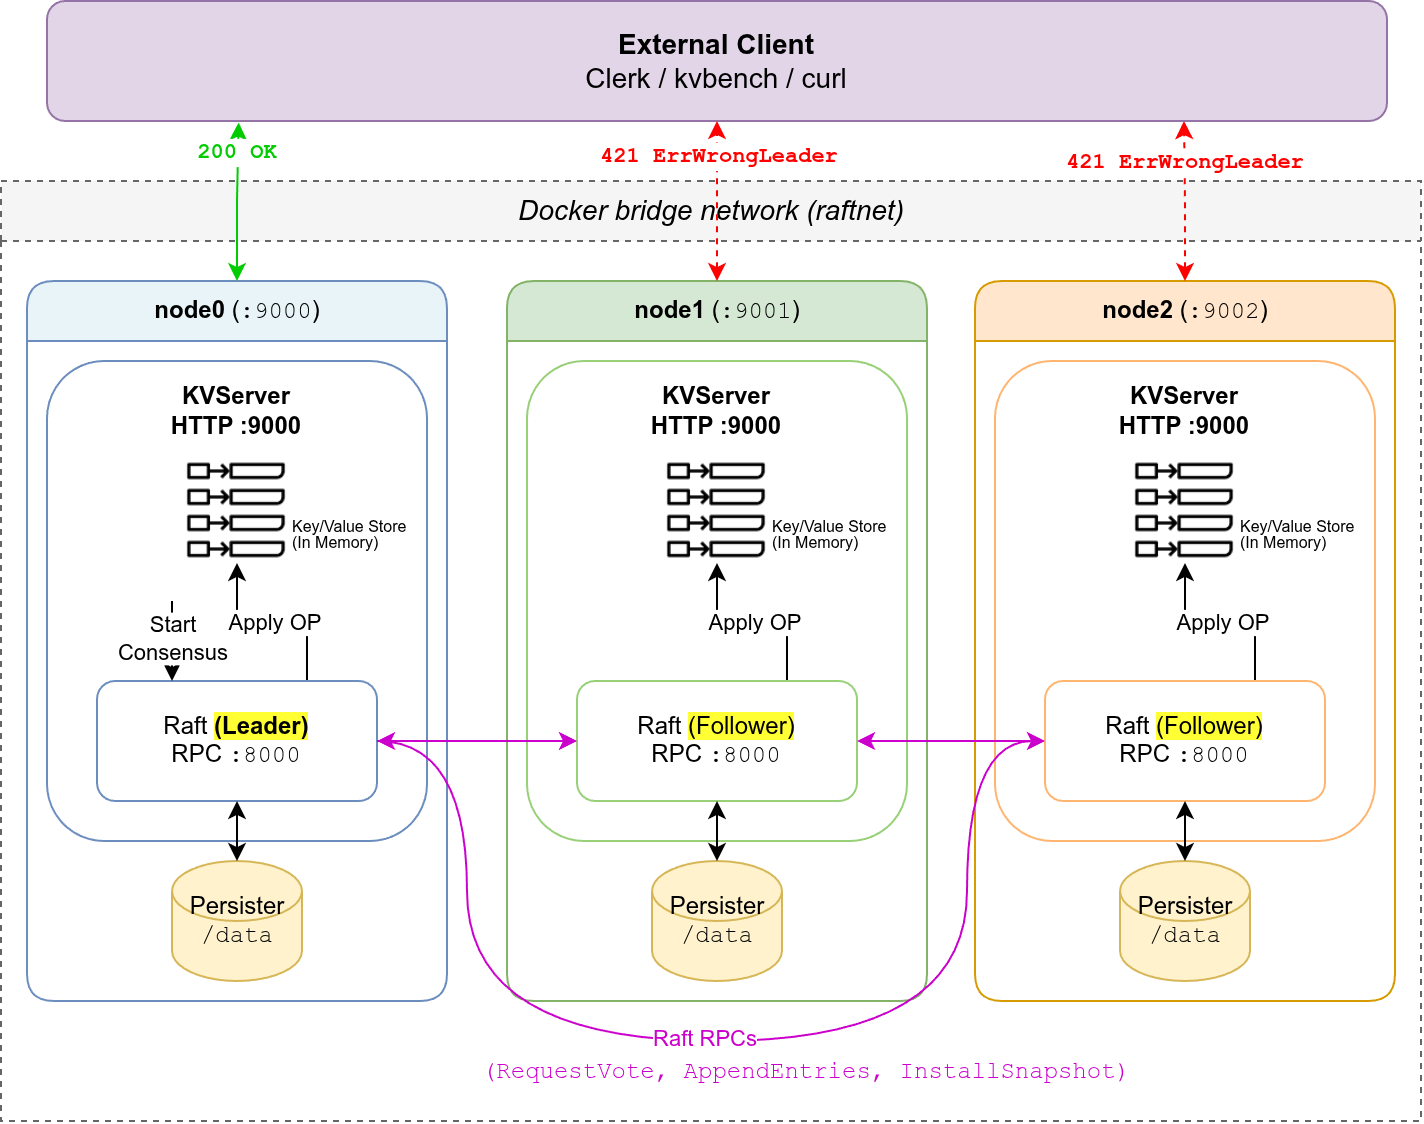
\includegraphics[width=\columnwidth]{figs/raft_kvstore_docker.png}
\caption{Containerized cluster architecture diagram.}\label{fig:arch}
\end{figure}

The nodes are configured through environment variables. The \texttt{compose.yaml} file on this project's repository contains an example of how to set these variables for a cluster of three nodes.

Clients have their own communication channel, separate from the one used by Raft, via HTTP over the endpoints described in Table~\ref{tab:endpoints}. Followers answer read and write requests with HTTP \texttt{421} and \texttt{ErrWrongLeader} rather than forwarding them, so leader discovery is entirely client-side.

The HTTP API also exposes a \texttt{/status} endpoint that reports useful state variables from the raft layer, including the term, the observed leader, the commit, last-log and applied indexes, and the sizes of the Raft state and snapshot; the experiments in Section~\ref{sec:method} poll it to derive the recovery metrics.

\begin{table}[h]
\centering
\small
\setlength{\tabcolsep}{4pt}
\caption{HTTP endpoints exposed by every node}\label{tab:endpoints}
\begin{tabular}{@{}llp{40mm}@{}}
\toprule
Method & Path & Effect \\
\midrule
GET  & \texttt{/status}     & node state: term, leader, indexes, state and snapshot sizes \\
GET  & \texttt{/kv/\{key\}} & read the value of a key \\
PUT  & \texttt{/kv/\{key\}} & set the key to the request body \\
POST & \texttt{/kv/\{key\}} & append the request body to the key \\
\bottomrule
\end{tabular}
\end{table}

Finally, each node persists its durable state to a mounted volume. The raft side persists the current term, vote and log, and the kvserver side persists the key/value map and the response cache.

\section{Correctness Properties and Tests}\label{sec:correct}
The Raft paper~\cite{raft2014} already proves that the protocol is safe, so our task was to make sure our code follows the rules that proof depends on, and to test that it does.

\subsection{Safety arguments}\label{sec:correct-safety}

\paragraph{One leader per term} A node grants at most one vote per term, and it saves \texttt{votedFor} and \texttt{currentTerm} to disk before answering a vote request,
so after a crash and restart it still knows whom it voted for and cannot vote again in the same term. A candidate needs votes from more than $N/2$ nodes, its own included.
Two leaders in the same term would need two such majorities, and any two majorities of the same $N$ nodes share at least one node, which would have had to vote twice (contradiction).

\paragraph{Log Matching} A leader never overwrites or deletes entries in its own log, only appends new ones, so it creates at most one entry per index in its term.
Each \texttt{AppendEntries} RPC carries the index and term of the entry right before the new ones, and the follower refuses the request unless it has that exact entry.
Every accepted request therefore extends a prefix that the follower already shares with the leader, and by induction, if two logs have an entry with the same index and term,
they agree on everything before it.

\paragraph{Committed entries are never lost} Since followers' logs are made to match the leader's, it suffices that every leader of a later term has all committed entries.
This follows from the election restriction: a node only votes for a candidate whose log is at least as up to date as its own, that is, whose last entry has a higher term than the voter's,
or the same term and an index at least as high. A committed entry is stored on a majority of nodes, and the new leader was voted in by a majority,
so at least one of its voters has the entry and would have refused a candidate without it. The Raft paper~\cite{raft2014} proves this formally, by induction over terms.

\paragraph{Same commands in the same order} \texttt{commitIndex} never decreases, and a single goroutine per node delivers entries to the service strictly in index order.
Together with the Log Matching property and the guarantee that committed entries are never lost, this means every replica applies the same command at each index,
so they all go through the same sequence of states.

\paragraph{Linearizability} Every client operation, \texttt{Get} included, is turned into a log entry, and the server only replies after that entry is applied.
The moment of application falls between the request and the reply, which is exactly the instant linearizability asks for.
Routing reads through the log also means that an old leader that was cut off cannot serve stale reads: it cannot commit anything, so its reads never succeed. The tricky part is the retries.
If a reply is lost, the \texttt{Clerk} sends the request again, possibly to another server, and the same command can end up in the log twice. Each server stores, for every client,
the \texttt{Seq} and result of the last operation it applied, and a request whose \texttt{Seq} is not newer than that gets the stored result instead of being applied a second time.
Since a \texttt{Clerk} has only one request in flight at a time, remembering the last one is enough.

\paragraph{Liveness} Unlike safety, liveness depends on timing, and holds only while a majority of nodes is up and can exchange messages within the timeouts. Under that condition,
randomized election timeouts make repeated split votes (elections in which no candidate gets a majority) unlikely. Once a leader is elected,
its heartbeats keep the followers from starting new elections while it retries \texttt{AppendEntries} until each entry is committed.

\subsection{Automated tests}\label{sec:correct-tests}

The 6.824 labs' tests run every peer inside a single Go process, connected through \texttt{labrpc}, a simulated in-memory network which gives the tester full control for injecting faults. It can disconnect a node, split the cluster into two partitions, or crash a node and later restart it from a copy of what it had persisted. It can also make the network unreliable with artificial delays and packet loss.

The Raft tests (2A--2C) are particularly strong, since safety is checked all the time, not only at the end. The tester records every entry that each peer applies, and fails immediately if two peers apply different commands at the same index, or if a peer applies an index before the previous one. Every time it looks for the leader, it also fails if it sees two leaders in the same term. So every Raft test, whatever it focuses on, is also checking that all replicas apply the same commands and that there is only one leader per term. The KV tests (3A--3B) look at the system from the outside instead, checking the values that clients get back. Every test also has a 120\,s limit, so an implementation that stays safe but takes too long to recover also fails. Table~\ref{tab:tests} lists the tests by part and how long they took to execute; Appendix~\ref{sec:correct-tests-detail} describes each one in detail. In short:

\begin{itemize}
\item \textbf{2A tests:} focus on leader election. They test whether raft elects exactly one leader, triggers a new election after the leader is disconnected, refuses to elect without a majority, and keeps a returning old leader from disturbing the new one.
\item \textbf{2B tests:} focus on log replication. They test whether raft commits with followers missing, and whether a leader overwrites long conflicting suffixes after partitions.
\item \textbf{2C tests:} focus on persistence. They crash and restart nodes in every relevant order, verifying correctness with clients writing while nodes fail and recover.
\item \textbf{3A tests:} focus on KV server functionalities by having concurrent clients append to and read their keys under an unreliable network with partitions and restarts.
\item \textbf{3B tests:} focus on snapshotting. They cap the persisted Raft state and snapshot size, and force a lagging server to catch up through \texttt{InstallSnapshot}.
\item \textbf{3A \& 3B linearizability tests:} use Porcupine to check the recorded client histories for a valid real-time ordering.
\item \textbf{Our test:} runs the deployed wiring (real TCP, HTTP, files on disk) through all KV Server operations.
\end{itemize}
All 40 individual tests pass.

\begin{table}[h]
\centering
\small
\caption{Automated tests and their running time}\label{tab:tests}
\setlength{\tabcolsep}{4pt}
\begin{tabular}{@{}llrr@{}}
\toprule
Part & Focus & Tests & Time (s) \\
\midrule
2A & leader election & 2 & 10.1 \\
2B & log replication & 8 & 62.2 \\
2C & persistence, Figure 8, churn & 8 & 129.3 \\
3A & KV service, linearizability & 13 & 249.3 \\
3B & snapshots & 8 & 152.5 \\
Ours & real TCP, HTTP and disk & 1 & 0.7 \\
\midrule
Total & & 40 & 604.1 \\
\bottomrule
\end{tabular}
\end{table}

\section{Experimental Methodology}\label{sec:method}
After verifying our implementation was correct, we set out to measure the performance cost of Raft's fault tolerance in our key/value service.

All experiments run on the containerized deployment of Section~\ref{sec:arch}, with every node on the same machine (Table~\ref{tab:env}). A single script, \texttt{scripts/run\_experiments.py}, runs every configuration of Section~\ref{sec:method-config}, each on a fresh cluster, and saves the raw results. \texttt{scripts/README.md} explains how to run it, and \texttt{scripts/analysis.ipynb} processes the raw results into the tables and figures of Section~\ref{sec:results}.

\begin{table}[h]
\centering
\small
\caption{Execution environment}\label{tab:env}
\begin{tabular}{@{}lp{50mm}@{}}
\toprule
Item & Value \\
\midrule
Hardware & Intel Core i5-1334U, turbo boost disabled; 7.6\,GiB RAM \\
Operating system & Windows 11, WSL2 (Linux 6.6.87.2) \\
Docker / Compose & 29.9.2 / 5.6.1 \\
Go / Python & 1.22.2 / 3.12.3 \\
Nodes & 3, 5, 7 containers (same host) \\
Load & 8 clients, 200 ops each \\
Seeds & 10 per configuration \\
Warm-up & 1 discarded run before the fault-free runs with 3, 5 and 7 nodes \\
\bottomrule
\end{tabular}
\end{table}

\subsection{Workload and scenarios}\label{sec:method-scenarios}
The load comes from \texttt{cmd/kvbench}, a small benchmark client that acts as the users of the key/value service. It runs eight clients, and each of them sends 200 operations,
waiting for the reply to one before sending the next. Half of the operations are writes and half are reads, all on the same five keys,
and at the end of each run \texttt{kvbench} checks the clients' history for linearizability with Porcupine.

We ran this load in four scenarios, chosen to cover the failures assumed in Section~\ref{sec:model}. The \emph{normal} scenario, where nothing goes wrong, gives us a reference.
In the \emph{delay and loss} scenario, \texttt{tc netem} is used to delay the packets that each container sends or to drop a fraction of them. In the \emph{crash} scenario,
we stop the leader's container (with \texttt{docker stop}), run the load on the remaining nodes once they have elected a new leader, and then restart the old leader, wait for it to catch up,
and run the load again on the full cluster. The \emph{partition} scenario follows the same steps, except that the leader is cut off from the network (with \texttt{docker network disconnect})
instead of stopped, and later reconnected.

In the crash and partition scenarios, we also measure how long the cluster takes to recover from the fault. For that, a separate client, the \emph{probe}, keeps writing from before the fault until the service returns, waiting for each write to finish before sending the next, and logs when each one starts and ends. Meanwhile, the experiment script asks every node for its Raft state through \texttt{/status} (Section~\ref{sec:arch}) every 50\,ms.

\subsection{Metrics}\label{sec:method-metrics}
For leader election, the main question is how long the cluster stays without a leader. From the node states we measure the \emph{time to elect},
which corresponds to the time from the fault occurring until some node reports being leader in a newer term. The probe gives us the time to recover service (\emph{TTR-service}):
the time from the fault until its first write that completes after it. It can be much longer than the election,
since a client whose request went to the old leader only tries another node after its client-side request timeout.

For log replication, the main question is what it costs to agree on every operation. This cost shows itself in the 50th, 95th and 99th latency percentiles (p50, p95, p99) of each run.
We also measure throughput, though the values we've measured have a different meaning than the usual: since each client waits for a reply before its next request,
the throughput is set by latency, not by how many requests the cluster could handle. After a crash or a partition, the node states also give us the time to recover a replica
(\emph{TTR-replica}), which is how long the returning node takes to apply everything the new leader had committed.

\subsection{Configurations}\label{sec:method-config}
Each parameter was tested at three levels while the other parameters kept their default value (no delay, no loss, three nodes): a delay of 0\,ms, 50\,ms or 100\,ms, a loss rate of 0\,\%, 2\,\% or 5\,\%, and clusters of 3, 5 or 7 nodes. The cluster size was varied not only in the normal scenario but also in the crash and partition scenarios. Each of these configurations ran with the same ten seeds, so all of them receive the same sequences of operations.

\section{Results}\label{sec:results}
\subsection{Throughput and Latency}

Table~\ref{tab:perf} shows a summary of the recorded throughput and latency for the tested scenarios. For raw results,
refer to the csv files in \texttt{scripts/experiments/*} in the project repository. All 200 runs, across every scenario, passed the linearizability check.

\begin{table}[h]
\centering
\small
\setlength{\tabcolsep}{4pt}
\caption{Throughput and per-operation latency without leader faults, median of ten seeds.}\label{tab:perf}
\begin{tabular}{@{}llr@{\hspace{12pt}}rrr@{}}
\toprule
 & & \emph{throughput} & \multicolumn{3}{c}{\emph{latency (ms)}} \\
\cmidrule(l){4-6}
Configuration & $N$ & ops/s & p50 & p95 & p99 \\
\midrule
No fault & 3 & 1671 & 4.5 & 7.1 & 9.1 \\
         & 5 & 1184 & 5.9 & 9.8 & 14.3 \\
         & 7 & 954 & 7.8 & 13.2 & 18.2 \\
50\,ms delay & 3 & 51 & 152 & 165 & 187 \\
100\,ms delay & 3 & 26 & 302 & 304 & 312 \\
2\,\% loss & 3 & 579 & 1.9 & 5.0 & 210 \\
5\,\% loss & 3 & 222 & 1.8 & 207 & 374 \\
\bottomrule
\end{tabular}
\end{table}

With no artificially injected network faults or delay, three nodes sustain 1671 ops/s. Growing the cluster appears to considerably worsen throughput,
with a 29\,\% drop from 3 to 5 nodes and a further 19\,\% from 5 to 7. Latency is also considerably affected.

Adding a 50\,ms delay on the network raises the median latency to 152\,ms, almost exactly three times the delay: one for each message a container sends per operation
(leader to follower, follower to leader, leader to client). Throughput falls to 51\,ops/s,
which matches the expected relationship of $\text{throughput} = N_\text{clients} / \text{latency} =8/0.152$. Doubling the delay doubles the effect on both numbers (302\,ms, 26\,ops/s).

Adding loss to the network did not raise the median latency (1.8--1.9\,ms, below the 4.5\,ms of the fault-free runs), but the occasional retransmissions show on the tail.
The p99 jumps from 9.1\,ms without faults to 210\,ms at 2\,\% loss and 374\,ms at 5\,\% loss.

\subsection{Recovery from a leader fault}

Table~\ref{tab:recovery} shows the mean recovery times from two possible leader faults: a crash and a network disconnect. Figure~\ref{fig:leader-fault} shows the timeline of one representative crash; throughput drops to zero at the fault and returns once the new leader is elected.

\begin{table}[h]
\centering
\footnotesize
\setlength{\tabcolsep}{3pt}
\caption{Recovery from a leader fault, mean $\pm$ stddev for ten seeds.}\label{tab:recovery}
\begin{tabular}{@{}llrrr@{}}
\toprule
Fault & $N$ & time-to-elect (ms) & TTR service (ms) & TTR replica (ms) \\
\midrule
Crash     & 3 & 1243 $\pm$ 1089 & 2405 $\pm$ 1184 & 584 $\pm$ 152 \\
          & 5 & 784 $\pm$ 36 & 2081 $\pm$ 461 & 526 $\pm$ 313 \\
          & 7 & 774 $\pm$ 47 & 2574 $\pm$ 1050 & 633 $\pm$ 270 \\
\midrule
Disconnect & 3 & 1571 $\pm$ 1380 & 3162 $\pm$ 1611 & 849 $\pm$ 447 \\
           & 5 & 911 $\pm$ 63 & 2494 $\pm$ 1054 & 1212 $\pm$ 1129 \\
           & 7 & 859 $\pm$ 30 & 2187 $\pm$ 27 & 780 $\pm$ 267 \\
\bottomrule
\end{tabular}
\end{table}

\begin{figure}[h]
\centering
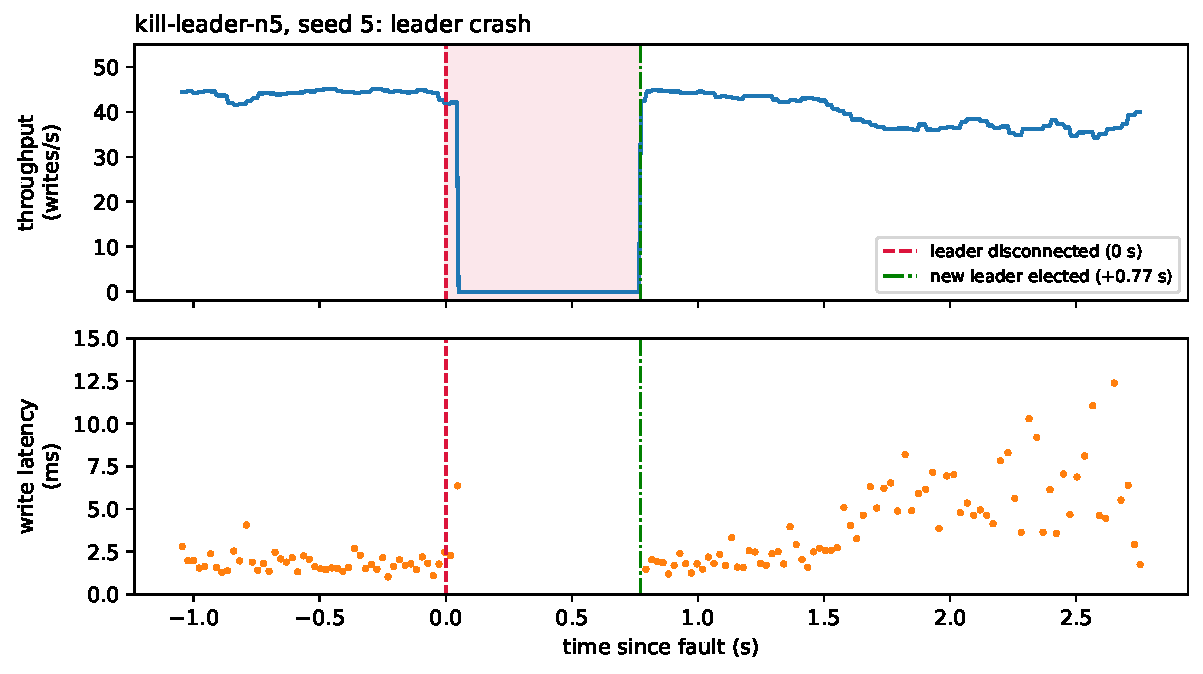
\includegraphics[width=\columnwidth]{figs/leader-fault-timeline.pdf}
\caption{One representative leader-crash run ($N=5$, seed 5): writes completed per second (top) and latency of each write (bottom).}\label{fig:leader-fault}
\end{figure}

The time to elect is much more stable with five and seven nodes than with three, for both faults. At three nodes, three runs took about 4\,s;
in all of them, two nodes stopped answering \texttt{/status} at the same time for over 3\,s in total, which points to a stall of the host or of Docker rather than of Raft.
Only one other slow run (2.0\,s) shows the extra term of a split vote. The typical election takes 0.8 to 0.9\,s, which matches the time the fault command takes to apply (about 0.3\,s),
the 500--700\,ms election timeout counted from the last heartbeat, and the 50\,ms polling resolution.

TTR-service averages between 2.1 and 3.2\,s across configurations. It also varies considerably between runs, except for partitions with seven nodes.
A possible explanation for this is that clients are set up to have 2\,s HTTP timeouts, and may or may not have to wait the full length of this timeout before searching for the new leader.

TTR-replica is somewhat stable for crashes, taking about 600\,ms. After a disconnection, it is noticeably larger.

\section{Limitations}\label{sec:limits}
In the Raft implementation, a new leader does not append the no-op entry that the paper prescribes at the start of each term~\cite{raft2014},
so entries from earlier terms are committed only when a client sends a new command. There is no ``PreVote'' and no ``check-quorum'' step when triggering elections,
so an isolated follower inflates its term and forces an election when it returns, and an isolated leader does not step down. The Raft state and the snapshot are written to two files,
each replaced atomically but not together, so a crash between the two writes can leave them out of step, and the replica may then lose operations that were already committed.
Finally, in our deployment setup, all nodes share one host, so they are not independent failure domains. It also affects the measurements: the network between containers is virtual,
so latencies are lower than between real machines, and all nodes compete for the same CPU and disk, which may account for part of the throughput drop as the cluster grows.

\section{Conclusion}\label{sec:conclusion}
This project set out to implement Raft with a key/value service on top of it and to measure the performance cost of its fault tolerance.
The implementation passes the whole MIT 6.824 test suite, and every one of the 200 experiment runs also passed the Porcupine linearizability check.

Taken together, the results point to a clear trade-off: replication buys availability, but latency and throughput suffer. Under normal operation,
three nodes sustained 1671\,ops/s with a median latency of 4.5\,ms. Growing to five nodes cost 29\,\% of the throughput, and to seven a further 19\,\%.
A network delay raised the median latency to about three times the injected delay, and packet loss did not raise the median but pushed the p99 from 9.1\,ms to as much as 374\,ms.
After a leader fault, a new leader was typically elected in 0.8 to 0.9\,s (over 2\,s in a few runs at $N=3$), and client-visible recovery took 2.1 to 3.2\,s,
likely dominated by the clients' 2\,s timeout.

Future work includes fixing the limitations of Section~\ref{sec:limits}, running the replicas on separate machines for more representative measurements,
and tuning the client timeout to shorten client-visible recovery.

\newpage
\appendices\section{Background: Raft}\label{sec:background}
A common way to build a fault-tolerant service is the \emph{replicated state machine}~\cite{vansteen2023}: every server keeps its own copy of the service state (in our case, a key/value map) and a log of commands. If all servers apply the same commands in the same order, all copies go through the same states and end up equal, so any of them can answer for the service (Figure~\ref{fig:raft-rsm}). The hard part is getting the servers to agree on the contents of the log while messages get lost and servers crash, which is a consensus problem. Raft~\cite{raft2014} solves it for a fixed group of $N$ servers, and keeps working as long as a majority of them (more than $N/2$) is up and able to talk to each other. A cluster of three servers survives one failure, and a cluster of five survives two.

\begin{figure}[h]
\centering
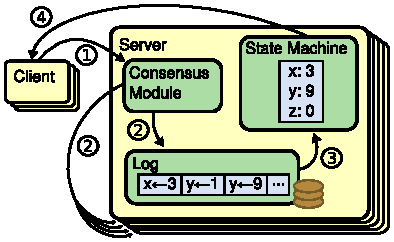
\includegraphics[width=\columnwidth]{figs/raft-fig1-rsm.pdf}
\caption{Replicated state machine architecture: the consensus module keeps a replicated log, and each state machine applies the same commands in the same order.
Adapted from Figure~1 of~\cite{raft2014}.}\label{fig:raft-rsm}
\end{figure}

\paragraph{Roles and terms} At any moment, each server is a \emph{follower}, a \emph{candidate} or the \emph{leader} (Figure~\ref{fig:raft-states}).
In normal operation there is exactly one leader, and the other servers are followers that only answer its requests. Time is divided into \emph{terms}, numbered with consecutive integers;
each term starts with an election and has at most one leader. Every message carries the sender's term, a server that sees a term higher than its own adopts it and becomes a follower,
and messages from older terms are rejected. This is how a leader that was cut off finds out that it has been replaced. The basic protocol needs only two RPCs,
\texttt{RequestVote} and \texttt{AppendEntries}. Optionally, an \texttt{InstallSnapshot} RPC is defined for log compaction.

\begin{figure}[h]
\centering
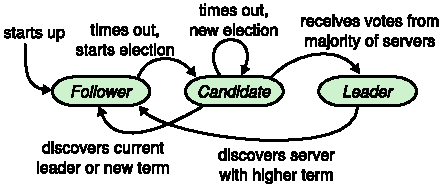
\includegraphics[width=\columnwidth]{figs/raft-fig4-states.pdf}
\caption{Raft server states and transitions. Adapted from Figure~4 of~\cite{raft2014}.}\label{fig:raft-states}
\end{figure}

\paragraph{Leader election} The leader sends periodic heartbeats (\texttt{AppendEntries} calls, possibly empty) to every follower. A follower that hears nothing for an \emph{election timeout} assumes the leader has failed: it increments its term, becomes a candidate, votes for itself and asks the other servers for their votes. Each server gives at most one vote per term, to the first candidate that asks, and only if that candidate's log is at least as up to date as its own. A candidate that gets votes from a majority becomes the leader and starts sending heartbeats. If the votes are split and nobody wins, the candidates time out and try again in a new term. Election timeouts are chosen at random, so this shouldn't happen many times in a row.

\paragraph{Log replication} Clients send their commands to the leader, which appends each one to its log as a new entry tagged with the current term, and sends it to the followers with \texttt{AppendEntries}. Each call also carries the index and term of the entry just before the new ones, and a follower only accepts it if its own log has a matching entry at that position. If not, the follower refuses, the leader retries from an earlier position, and once the two logs match, the follower's conflicting entries are replaced by the leader's. When an entry is stored on a majority of servers, the leader considers it \emph{committed}, applies it to its state machine and answers the client service. Followers learn the new commit index from later \texttt{AppendEntries} calls and apply the entry too.

\paragraph{Persistence and snapshots} Each server saves its current term, its vote and its log to stable storage before answering any RPC, so that it can crash, restart and rejoin without breaking promises it made before the crash. Since the log would otherwise grow forever, the service periodically saves a \emph{snapshot} of its state, and Raft throws away the log entries that the snapshot covers. A follower that is so far behind that the leader no longer has the entries it needs receives the leader's snapshot through \texttt{InstallSnapshot}.

\section{Reused Code and Modifications}\label{sec:algs-reuse}
All the code we reused comes from the framework of MIT's 6.824 course (2020)~\cite{mit6824}, specifically labs 2 and 3.

The starting point was the stubs in \texttt{raft.go}, \texttt{server.go}, \texttt{client.go} and \texttt{common.go}, which define the API that the tests call (\texttt{Make}, \texttt{Start},
\texttt{GetState}, \texttt{StartKVServer}, the \texttt{Clerk} methods and the RPC argument types). We kept that API and wrote everything behind it.
Among the elements kept as they were are the simulated in-memory network (\texttt{labrpc}), the gob wrapper (\texttt{labgob}), the Porcupine checker~\cite{porcupine} with its key/value model,
and the test suites (\texttt{test\_test.go}) with their harnesses (\texttt{config.go}), in both \texttt{src/raft} and \texttt{src/kvraft}, apart from the first change below.

We made two small changes to the labs' skeleton.
The one-method \texttt{RPCClient} interface was added to \texttt{labrpc}, and the test harnesses were made to use it instead of the concrete \texttt{*labrpc.ClientEnd} type,
which changes no test logic but allows switching between the simulated in-memory network of the tests and the TCP transport used in deployment.
We also gave the \texttt{Persister} an optional file-backed mode (\texttt{MakeFilePersister}), used only in deployment, while the tests still use the in-memory version.

Everything else was written by us: the Raft implementation (about 1{,}000 lines in \texttt{raft.go}), the KV server and \texttt{Clerk}, the TCP transport (\texttt{labrpc/tcp.go}),
the HTTP API with \texttt{/status} and \texttt{HTTPEnd} (\texttt{kvraft/http.go}), the node binary (\texttt{cmd/kvnode}), the benchmark client (\texttt{cmd/kvbench}),
our \texttt{TestHTTPAndTCPCluster} test, the \texttt{Dockerfile} and \texttt{compose.yaml}, and the experiment scripts.

\section{Automated Tests: Detailed Descriptions}\label{sec:correct-tests-detail}
\paragraph{2A tests (leader election)} \texttt{InitialElection} checks that three nodes elect exactly one leader and agree on its term, and that the leader is still there two seconds later. \texttt{ReElection} disconnects the leader and expects a new one to be elected. The old leader coming back must not disturb the new one, with two of the three nodes disconnected no leader may be elected, and once a majority is back, one must be.

\paragraph{2B tests (log replication)} Here commands are submitted with \texttt{Start} and must be committed at the expected index by the expected number of nodes.
\texttt{FailAgree} keeps committing with one follower disconnected and checks that it catches up when it comes back,
while \texttt{FailNoAgree} checks that nothing commits when three of five followers are gone. In \texttt{Rejoin}, a disconnected leader accepts entries that can never commit,
and when it reconnects it must drop them in favor of the new leader's log. \texttt{Backup} pushes this further: two minority partitions each pile up 50 uncommitted entries,
and then nodes are reconnected in other combinations, so the leader has to overwrite long conflicting suffixes on its followers.
\texttt{ConcurrentStarts} calls \texttt{Start} from several goroutines at once. Finally, \texttt{RPCBytes} and \texttt{Count} test for excessive communication,
making sure that each command is sent about once to each follower, an election may take at most 30 RPCs, and one idle second at most 60 RPCs.

\paragraph{2C tests (persistence)} The three \texttt{Persist} tests crash and restart nodes in different orders (all of them, only the leader, a follower while the others keep committing, a partitioned leader together with a follower), and a restarted node must come back with its term, vote and log. \texttt{Figure8} recreates the scenario behind the current-term commit rule: for 1000 iterations it gives a command to the leader and crashes it shortly after, usually before the entry commits, and restarts nodes whenever fewer than three are up. \texttt{Figure8Unreliable} does the same with disconnections instead of crashes, on an unreliable network, and turns on long reordering after 200 iterations. \texttt{UnreliableAgree} commits commands concurrently over the lossy network. The two \texttt{Churn} tests have three clients submitting commands while nodes are randomly disconnected, crashed and restarted every 700\,ms; at the end, every value that a client saw committed must be in the final log of every node.

\paragraph{3A tests (KV service)} Most of these tests share the same routine, with five servers and three rounds of five seconds, in which each client appends to and reads its own key. Since each client is the only writer of its key, it knows what every \texttt{Get} must return, and any other value fails the test. After each round, every key is read back and each append must appear exactly once and in order, so both a lost write and a duplicate caused by a retry are caught. Options add more clients (five instead of one), an unreliable network, a partitioner that splits the servers into two random groups about once per second, and a restart of every server at the end of each round. \texttt{UnreliableOneKey} has five clients appending to the same key over the lossy network. \texttt{OnePartition} puts the leader on the minority side of a partition. The majority must keep serving requests, a \texttt{Put} and a \texttt{Get} sent to the minority must not complete, and the \texttt{Put} must go through once the partition heals. The \texttt{Get} on the minority side is the one that would catch an old leader serving stale reads.

\paragraph{3B tests (snapshots)} These tests set \texttt{maxraftstate} to 1000 bytes and, after each round, require the persisted Raft state to be at most eight times that, which means the log is really being trimmed. In \texttt{SnapshotRPC}, one server falls behind in a minority while the other two commit 50 writes and compact their logs. The partition then changes so that the lagging server is needed for a majority, and the only way it can catch up is through \texttt{InstallSnapshot}, since the leader has already thrown away the entries it is missing. \texttt{SnapshotSize} requires snapshots smaller than 500 bytes after 800 operations on a single key. The other six tests repeat the 3A combinations of faults, with up to 20 clients, with snapshots turned on.

\paragraph{3A \& 3B tests on linearizability} There are two \emph{Linearizable} tests, one in 3A and one in 3B. Fifteen clients send random \texttt{Put}, \texttt{Append} and \texttt{Get} requests on shared keys to seven servers, with lossy network, partitions and restarts all active, and the start and end time of every operation is recorded. Porcupine~\cite{porcupine} then searches for a single order of all the operations that respects real time (if one operation returned before another started, it must come first) and that explains every value returned by a \texttt{Get}. If no such order exists, the history is not linearizable and the test fails.

\paragraph{Our own test} All inherited tests use \texttt{labrpc} and the in-memory persister, so none of them runs the code that is used in the containers. To cover it,
we wrote \texttt{TestHTTPAndTCPCluster}, which starts three nodes wired the same way as in the deployment: Raft over \texttt{net/rpc} on real TCP sockets, state saved to files on disk,
and clients talking HTTP\@. It runs a \texttt{Put}, an \texttt{Append} and a \texttt{Get} through the \texttt{Clerk} and then checks three things:
followers answer a write with HTTP 421 instead of applying it, \texttt{/status} reports the same leader on every node,
and every node has $\textit{lastApplied} \le \textit{commitIndex} \le \textit{lastLogIndex}$. This is only a smoke test without faults;
the experiments of Section~\ref{sec:method} are what exercise the deployment under faults.

\bibliographystyle{IEEEtran}
\bibliography{refs}

\end{document}
